\documentclass[a4paper,11pt]{article}

\usepackage{url}
\usepackage{graphicx}
\usepackage{enumerate}
\usepackage{amsmath}
\usepackage{float}
\usepackage{longtable}
%\usepackage{fullpage}
\usepackage{pstricks}
\usepackage{tikz}
\usepackage[absolute]{textpos}
\usepackage{import}
\usepackage{subfigure}
\usepackage{setspace}

\title{G53NMD Individual Assignment}
\author{Robert J. Golding (rjg08u)} \date{\today}

% Dutch style paragraph formatting
\setlength{\parskip}{1.3ex plus 0.2ex minus 0.2ex}
\setlength{\parindent}{0pt}

%\doublespacing
\onehalfspacing

\begin{document}
    \maketitle

    \begin{quote}
        \emph{Social media on a mobile platform is the pinnacle of excellence
        of new media. Discuss with examples the validity of this statement and
        how these technologies have changed the nature of design.}
    \end{quote}

    \section{Introduction}

    To understand what Social media is (and also what it is \emph{not}), one
    must first get a feel for the related topics: Web 2.0 and User Generated
    Content. \cite{kaplan2010}

    Web 2.0 is a term that was first used in 2004 to describe a new way in
    which developers and end-users were starting to use the internet. It refers
    to the move away from the traditional model whereby content was created and
    published by individuals, remaining relatively static from that point on.
    Instead, the web became a collaborative platform upon which content could
    be continuously modified by users themselves.

    Though Web 2.0 does not refer to any particular technical ``update'' of the
    web itself, there are certain underlying technologies that are required for
    it to function. Among these are Adobe Flash---allowing videos, audio, and
    other forms of multimedia to be added to web pages---and RSS (Really Simple
    Syndication)---a method for retrieving content that is updated frequently,
    such as blog entries or news headlines.

    User Generated Content refers to, quite simply, content that has been
    generated by the \emph{users} of the web. According to the Organisation for
    Economic Co-operation and Development \cite{vickery2007}, user generated
    content must fulfill three requirements to be considered as such. It must:

    \begin{itemize}
        \setlength{\parskip}{0pt}
        \item be published on a publicly accessibly website (or social
            networking website accessible to selected users);
        \item show a certain amount of creative effort (i.e. not be a direct
            re-publication of another work);
        \item have been created outside of professional routines and practices.
    \end{itemize}

    Though User Generated Content has been around prior to the rise of Web 2.0,
    the combination of technological, economic and social drivers make it more
    pervasive and different from that which was observed in the first instance.

    Given these definitions, Social Media can be described as a group of
    internet based application that build upon the foundations of Web 2.0,
    allowing the creation and exchange of User Generated Content
    \cite{kaplan2010}.

    New media, meanwhile, has a different, wider meaning. Also, new media is
    a difficult term to define due to the extremely blurred line between
    ``new'' and ``old''. New media captures the development of new technologies
    (most notably the internet), and the remaking of more traditional forms of
    media \cite{flew2008}. The internet is the newest, most significant
    manifestation of new media, allowing information and \emph{knowledge} to be
    published and shared in ways and, indeed, at a speed never before
    possible.

    \section{Mobile Platforms}

    Recent advances in technology have seen content previously only available
    to desktop computers become available to mobile devices also. This owes to
    the increasing power and decreasing size of mobile devices, and the
    widespread availability of mobile internet through 3G and/or WiFi networks.

    Social media on a mobile platform changes the very nature of the media
    itself. Instead of something which is considered a separate task,
    interacting with social media becomes part of one's daily life. The ability
    to access services such as Facebook, Twitter or FourSquare whilst not sat
    at a desk is a nothing short of a revolution in computing history
    \cite{smith2009}.

    One important aspect of social media, particularly on a mobile platform, is
    that it breaks down boundaries. Whether those boundaries are social,
    economic, geographic or political, social media makes it possible for
    people to interact and communicate like never before.

    \section{The Revolution}

    The way people use the web today is completely different
    from that of just 10 years ago. The web is now an interactive experience,
    with almost every page inviting users to ``share'' content with their
    online friends via social networking platforms and respond to content with
    their own opinions \cite{smith2009}.

    Social media has contributed to change in the world in many ways. Recently,
    however, that has been more true then ever with the protests in North
    Africa and the Middle East.

    Though Egypt has long been considered a centre of stability in a volatile
    region, this view masked malignant problems which had simmered for years.
    The anti-government sentiment erupted in a series of protests in January
    when demonstrators marched against the 30-year rule of the then-president
    Honsi Mubarak.

    Even though the protesters had no clear leader, they were able to organise
    large numbers of people at very short notice across the country, leveraging
    social platforms such as Twitter, Facebook and YouTube to communicate.

    In fact, the Egyptian authorities saw mobile social media as such a threat,
    mobile towers were shut down in several areas, effectively preventing the
    protesters from communicating with one-another. Residents, however,
    responded by removing the encryption keys to their WiFi networks, allowing
    the crowds to use their internet connections to circumvent the block.

    Social media has become such an important factor in politics, particularly
    in the middle-east, that the Al Jazeera news organisation has launched
    a ``Twitter dashboard'' to track events in Bahrain, Egypt, Libya, Syria and
    Yemen.

    This is an example of how social media, particularly in the mobile form, is
    changing the world we live in. It isn't just altering individuals'
    perspectives, though. Increasingly, content published by users themselves
    is being used in reports by highly regarded news organisations such as the
    BBC. This was exemplified in the recent raid in Abbottabad which resulted
    in the killing of Osama Bin Laden, America's most wanted man.

    During the raid, a Pakistani IT consultant living in the town posted
    several messages to his Twitter account, reporting U.S. helicopters flying
    overhead---and subsequently one crashing. Obviously, the raid was not known
    to the public prior to its occurrence, so the Twitter user, Sohaib Athar,
    had no idea what he was experiencing at the time.

    Ultimately, this led to the world's media hearing about the raid---and much
    speculation as to its purpose---well before the government made an
    announcement. Mr Athar's tweets were used in mainstream media reports, and
    received widespread coverage from journalists around the world. Prior to
    the introduction of social media into the daily lives of the general
    public, events such as this would have gone unreported until
    after-the-fact. So, the time taken for the international community to learn
    of these events, and subsequently respond, would have been much longer.

    In this way, social media on a mobile platform has contributed to not only
    a revolution in new media, but also the wider world.

    \section{Concerns}

    The events in Libya and Pakistan represent a shift in the way news is
    gathered and reported.  Apparently, though, it's not all good. On the BBC's
    \emph{NewsWatch} programme, where viewers are given the chance to voice
    their concerns about BBC News, a number of people raised the issue of
    social media. Viewers were concerned about the use of ``unverified''
    footage taken by members of the public, and believed that the viewpoint
    presented was biased. Indeed, without careful consideration as to the
    validity of all sources---not just social media---there is a risk of false
    information being reported as fact.

    However, one could also argue that the benefits of social media in the news
    outweigh the risks. Often, events unfold so quickly that news crews don't
    have time to travel to the physical location fast enough. In cases such as
    this, footage taken by members of the public can provide a unique and
    otherwise unseen viewpoint.

    Also, people are increasingly posting personal, potentially damaging
    information on social networking websites such as Facebook, without
    realising the implications. Embarrassing photographs have become
    commonplace on the profiles of young people, particularly students. This
    type of content, though, can often cause serious damage to future career
    prospects now that employers so frequently ``Google'' prospective
    candidates.

    \section{New Media and Technology}

    \begin{figure}
        \begin{center}
            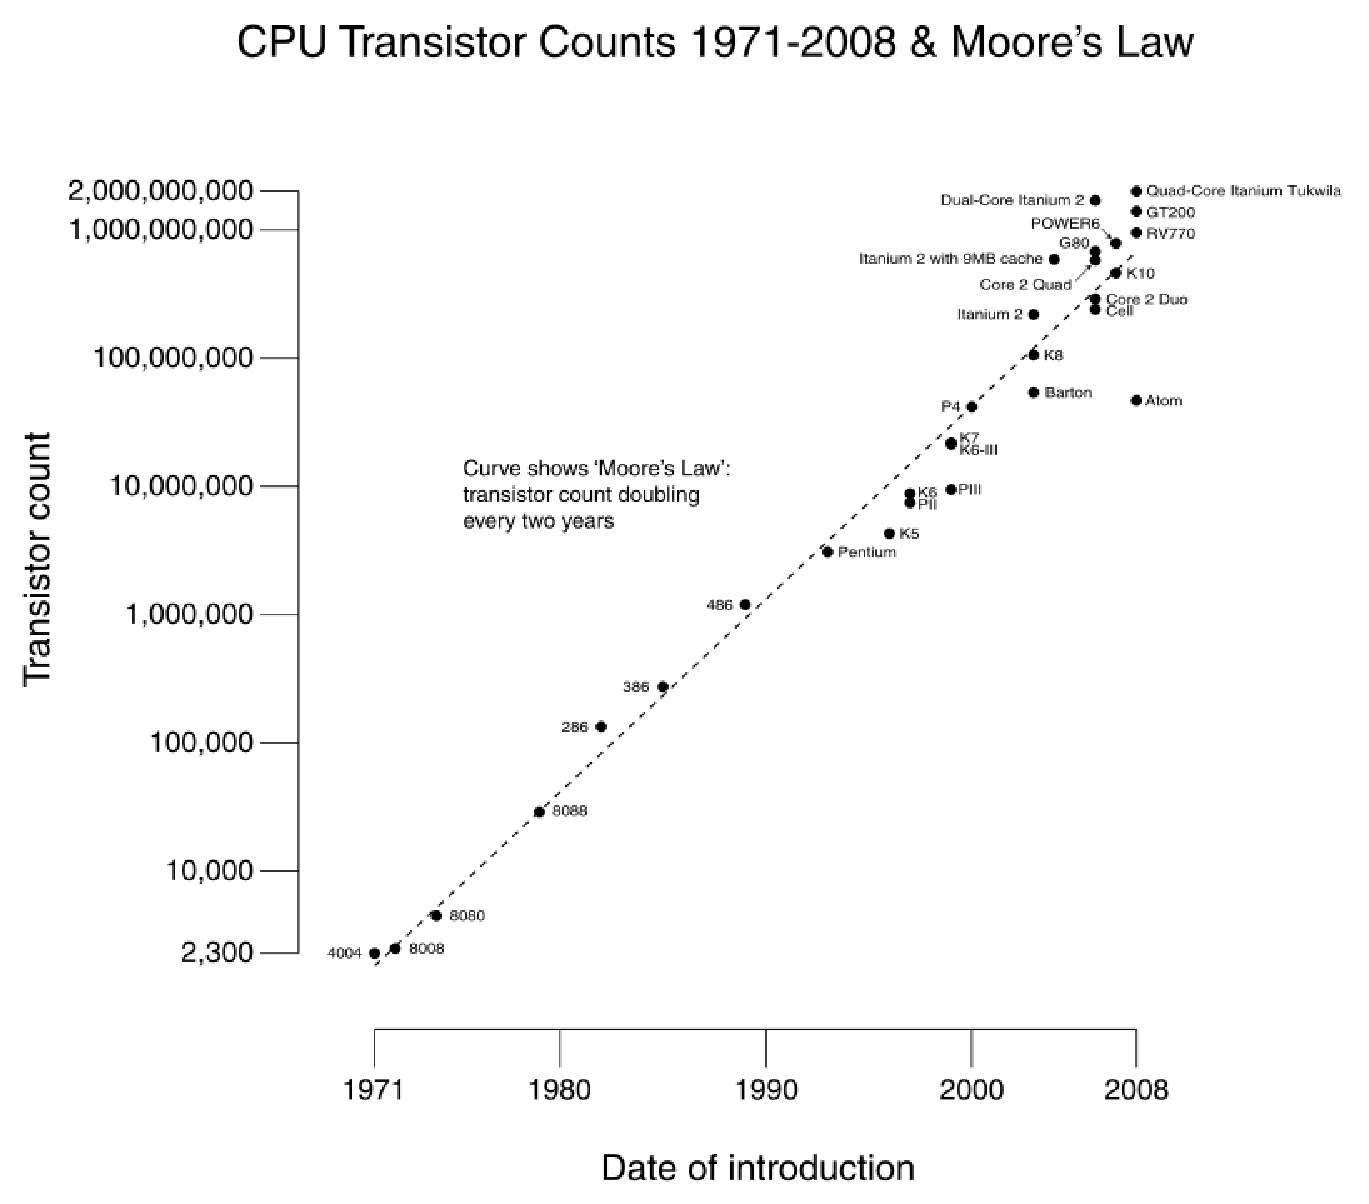
\includegraphics[width=\textwidth]{moores-law}
        \end{center}
        \caption{Graph illustrating Moore's Law: CPU transistor counts doubling
        every 2 years}
        \label{fig:moores-law}
    \end{figure}

    Moore's law states that, effectively, computing power doubles every 24
    months as the number of transistors which can be placed on an integrated
    circuit of a certain size multiplies \cite{schaller1997}. Figure
    \ref{fig:moores-law} shows that this trend has continued for almost half
    a century, and it is expected to continue until 2020 \cite{kanellos2005}.
    The exponential growth in computing power has enabled advanced technologies
    such as social media to become available on ever smaller devices.

    This means that today's mobile smart phones and tablets are, and will
    continue to be, smaller and more powerful than ever before. This rapid
    advance in technological capability has allowed developers to leverage the
    ever-increasing power of devices, even in the users' pockets.

    As an example, Foursquare is a service which allows users to ``check-in''
    to their current location over the internet, determined via the GPS chip on
    their mobile device. In this way, Foursquare makes use of many of the most
    recent advances in mobile technology.

    Without the improvements in mobile technologies such as faster, smaller
    CPUs and low-power GPS chips, services such as Foursquare would not be
    a reality. The demand for such services, and the ever-changing requirements
    of social media, drive the change in mobile technology---challenging
    hardware manufacturers to keep pace. In this way, social media ``gone
    mobile'' is changing the design of hand-held devices to facilitate
    ever-more creative ways of allowing users to interact with online services.

    Although mobile technology is constantly being shifted by the increasingly
    demanding requirements of social media in the modern age, we have reached
    a point whereby computers impact upon every part of our daily lives.
    Smart-phones are now small enough, and have batteries which last long
    enough, to be used at all times and in all places throughout the day.
    Though \emph{ubiquitous computing} promises to further integrate computers
    into the fabric of our lives, the core concepts and technologies remain the
    same.

    \section{New Media and Design}

    In parallel with the quickly shifting world of mobile technologies, the
    design of user interfaces must also adapt to suit not only the platform
    they are targeted at, but also the type of interaction that is required. As
    the web becomes more and more interactive, the act of browsing the web has
    become a much less passive affair. The traditional way of accepting user
    input through buttons and forms is adapting to cope with this change.

    For example, Facebook recently changed the way in which comments are posted
    on their pages. Instead of filling in a form and then clicking a ``submit''
    button, users now simply type their comment on the page itself. When they
    press enter, the comment is published immediately without refreshing the
    page. This seemingly minor change has the effect of increasing the speed at
    which users are able to interact with the website, and encourages even more
    engagement.

    With regards to mobile platforms, the entire user experience has had to be
    redefined, owing to the new way in which users interact with the interface
    itself. Mobile devices, typically, have touch-sensitive screens, with
    little or no physical buttons. This means that the traditional style of
    user interface is not suitable for use on mobile platforms.

    Interfaces which are designed to be used on a touch-screen mobile device
    will typically need larger, easy-to-hit buttons and a larger, clearer
    typeface \cite{gong2004}. Also, users should be able to use shortcuts for
    frequently performed actions, and the navigation structure should be very
    simple. Often, the lack of physical buttons causes an issue for interface
    designers - as they must strive to make every available action doable via
    touch-sensitive buttons on the screen, taking up vital real-estate
    \cite{brewster2002}.

    \section{Summary}

    The design of mobile devices, along with the underlying technology, is
    constantly changing and adapting to meet the demands of users, and the
    services themselves. User interface design must also keep up with this
    change, however, to ensure that services remain accessible no matter what
    platform they are accessed from.

    \bibliographystyle{alpha}
    \bibliography{references}

\end{document}
